\documentclass[runningheads]{llncs}
%
\usepackage[T1]{fontenc}
\usepackage{lmodern}

\ifdefined\pdfgentounicode
  \input{glyphtounicode}
  \pdfgentounicode=1
  \pdfminorversion=7
\fi
\usepackage{graphicx}
\usepackage{amsmath,amssymb}
\usepackage{booktabs}
\usepackage{url}
\usepackage{placeins}
%
\begin{document}
%
\title{Interval Selection for Adversarial Rank Suppression in Windowed Text-to-Video Retrieval}
\titlerunning{Interval Selection for Adversarial Rank Suppression}
%
\author{Nhat Lam Phuong Phan\inst{1} \and
Ngoc Hoang Luong\inst{1}}
\authorrunning{N. L. P. Phan and N. H. Luong}
%
\institute{University of Information Technology, Ho Chi Minh City, Vietnam\\
Vietnam National University, Ho Chi Minh City, Vietnam\\
\email{25521478@gm.uit.edu.vn, hoangln@uit.edu.vn}}
%
\maketitle

% Preserve LNCS running heads without page numbers for submission.
\pagestyle{headings}
\makeatletter
\def\@evenhead{\normalfont\small\hspace{\headlineindent}\leftmark\hfil}
\def\@oddhead{\normalfont\small\hfil\rightmark\hspace{\headlineindent}}
\makeatother
\thispagestyle{empty}
%
\begin{abstract}
We study white-box adversarial rank suppression in text-to-video retrieval under a budget of 16 consecutive editable keyframes and an $\ell_\infty$ pixel bound of $8/255$. In the evaluated system, a video's score is determined by its highest-scoring temporal window. Editing one matching scene may therefore have little effect if another strong match remains unchanged. We evaluate an interval-selection rule that minimizes the highest score among windows outside the editable interval. Evaluation covers 141 queries across two rounds: an initial 48-query evaluation and a 93-query extension whose configuration was locked before its attack results were observed. Both rounds use the same fixed collection of 873 videos. Compared with target-centered and highest-score-window selection under the same optimizer and pixel budget, our rule improves average target-rank suppression in both rounds, with frequent ties against highest-score-window selection. These results show that accounting for unaffected windows can strengthen rank suppression under a limited edit budget.
\keywords{Video retrieval \and Adversarial attack \and Known-item search
\and Vision-language model \and Temporal window selection}
\end{abstract}
%
\section{Introduction}

Text-to-video known-item retrieval aims to locate a specific video in a collection from a natural-language query. We study a white-box attack that suppresses the target video's rank by perturbing one interval of 16 consecutive sampled keyframes. The perturbations are bounded in pixel space, while the query, retrieval model, and all other videos remain fixed.

The evaluated retriever scores overlapping temporal windows and assigns each video its maximum window score. This aggregation makes interval selection important: suppressing one matching scene may leave the video score largely unchanged if another high-scoring window remains unaffected.

We select the editable interval by considering the windows that it cannot affect. For each candidate interval, we compute the maximum clean score among non-overlapping windows, called the \emph{unaffected floor}. We choose the interval that minimizes this value and then apply pixel optimization. This criterion accounts for competing temporal matches before allocating the perturbation budget. Our focus is the placement of contiguous edits under maximum window aggregation; the pixel optimizer and temporal regularizer are shared controls rather than new attack components.

\noindent Our contributions are:\nopagebreak
\begin{itemize}
\item an analysis of how unaffected temporal windows limit local score suppression under maximum aggregation;
\item an interval-selection rule that minimizes the maximum clean score among unaffected windows; and
\item a controlled comparison of three interval selectors in two rounds of 48 and 93 queries, with full-corpus ranking, paired statistical analysis, and image-quality measurements; the 93-query extension was locked before its attack results were observed.
\end{itemize}


\section{Related Work}

\subsection{Adversarial attacks on video models}

Video adversarial attacks must account for both the temporal support and temporal structure of perturbations. Wei et al.~\cite{wei2019sparse} study perturbations that affect only selected frames. Pony et al.~\cite{pony2021flickering} study temporally structured changes and penalize large first- and second-order differences between frames. These video-recognition studies motivate controlling both the number of modified frames and the temporal variation of perturbations.

\subsection{Selecting frames to attack}

Search-and-Attack~\cite{heo2021search} separates frame selection from pixel optimization and uses gradient information to find vulnerable frames. Xu et al.~\cite{xu2022keyframe} also choose important frames before generating an attack. These methods establish selection before optimization, with frame subsets that need not form one contiguous interval. Their goal is to identify frames that strongly affect a video classifier. Our setting is different: the retriever scores many overlapping windows and keeps their maximum. We therefore select one contiguous interval by examining the strong windows that the interval cannot change.

Yao et al.~\cite{yao2025duo} propose DUO, a targeted black-box attack that sparsifies edits across frames and pixels of a query video. Their video-to-video setting differs from ours, where a text query remains fixed and the attacker edits one contiguous interval in a target video from the collection.

\subsection{Attacks on video-text retrieval}

Yang et al.~\cite{yang2024vtra} propose white-box and black-box attacks on video-text retrieval. Tian et al.~\cite{tian2025vipro} study the related task of promoting a video for multiple queries. Our contribution concerns where to place a fixed contiguous edit interval when video scores are maxima over overlapping windows. We compare internal interval selectors under the same pixel optimizer and perturbation budget. This isolates interval placement; it does not constitute a reproduction of, or a performance comparison against, these published attacks.

\section{Method}

The attack consists of temporal window scoring, interval selection, constrained pixel optimization, and full-corpus reranking. Figure~\ref{fig:attack-framework} illustrates the pipeline using a development example.

\begin{figure}[!htbp]
\centering
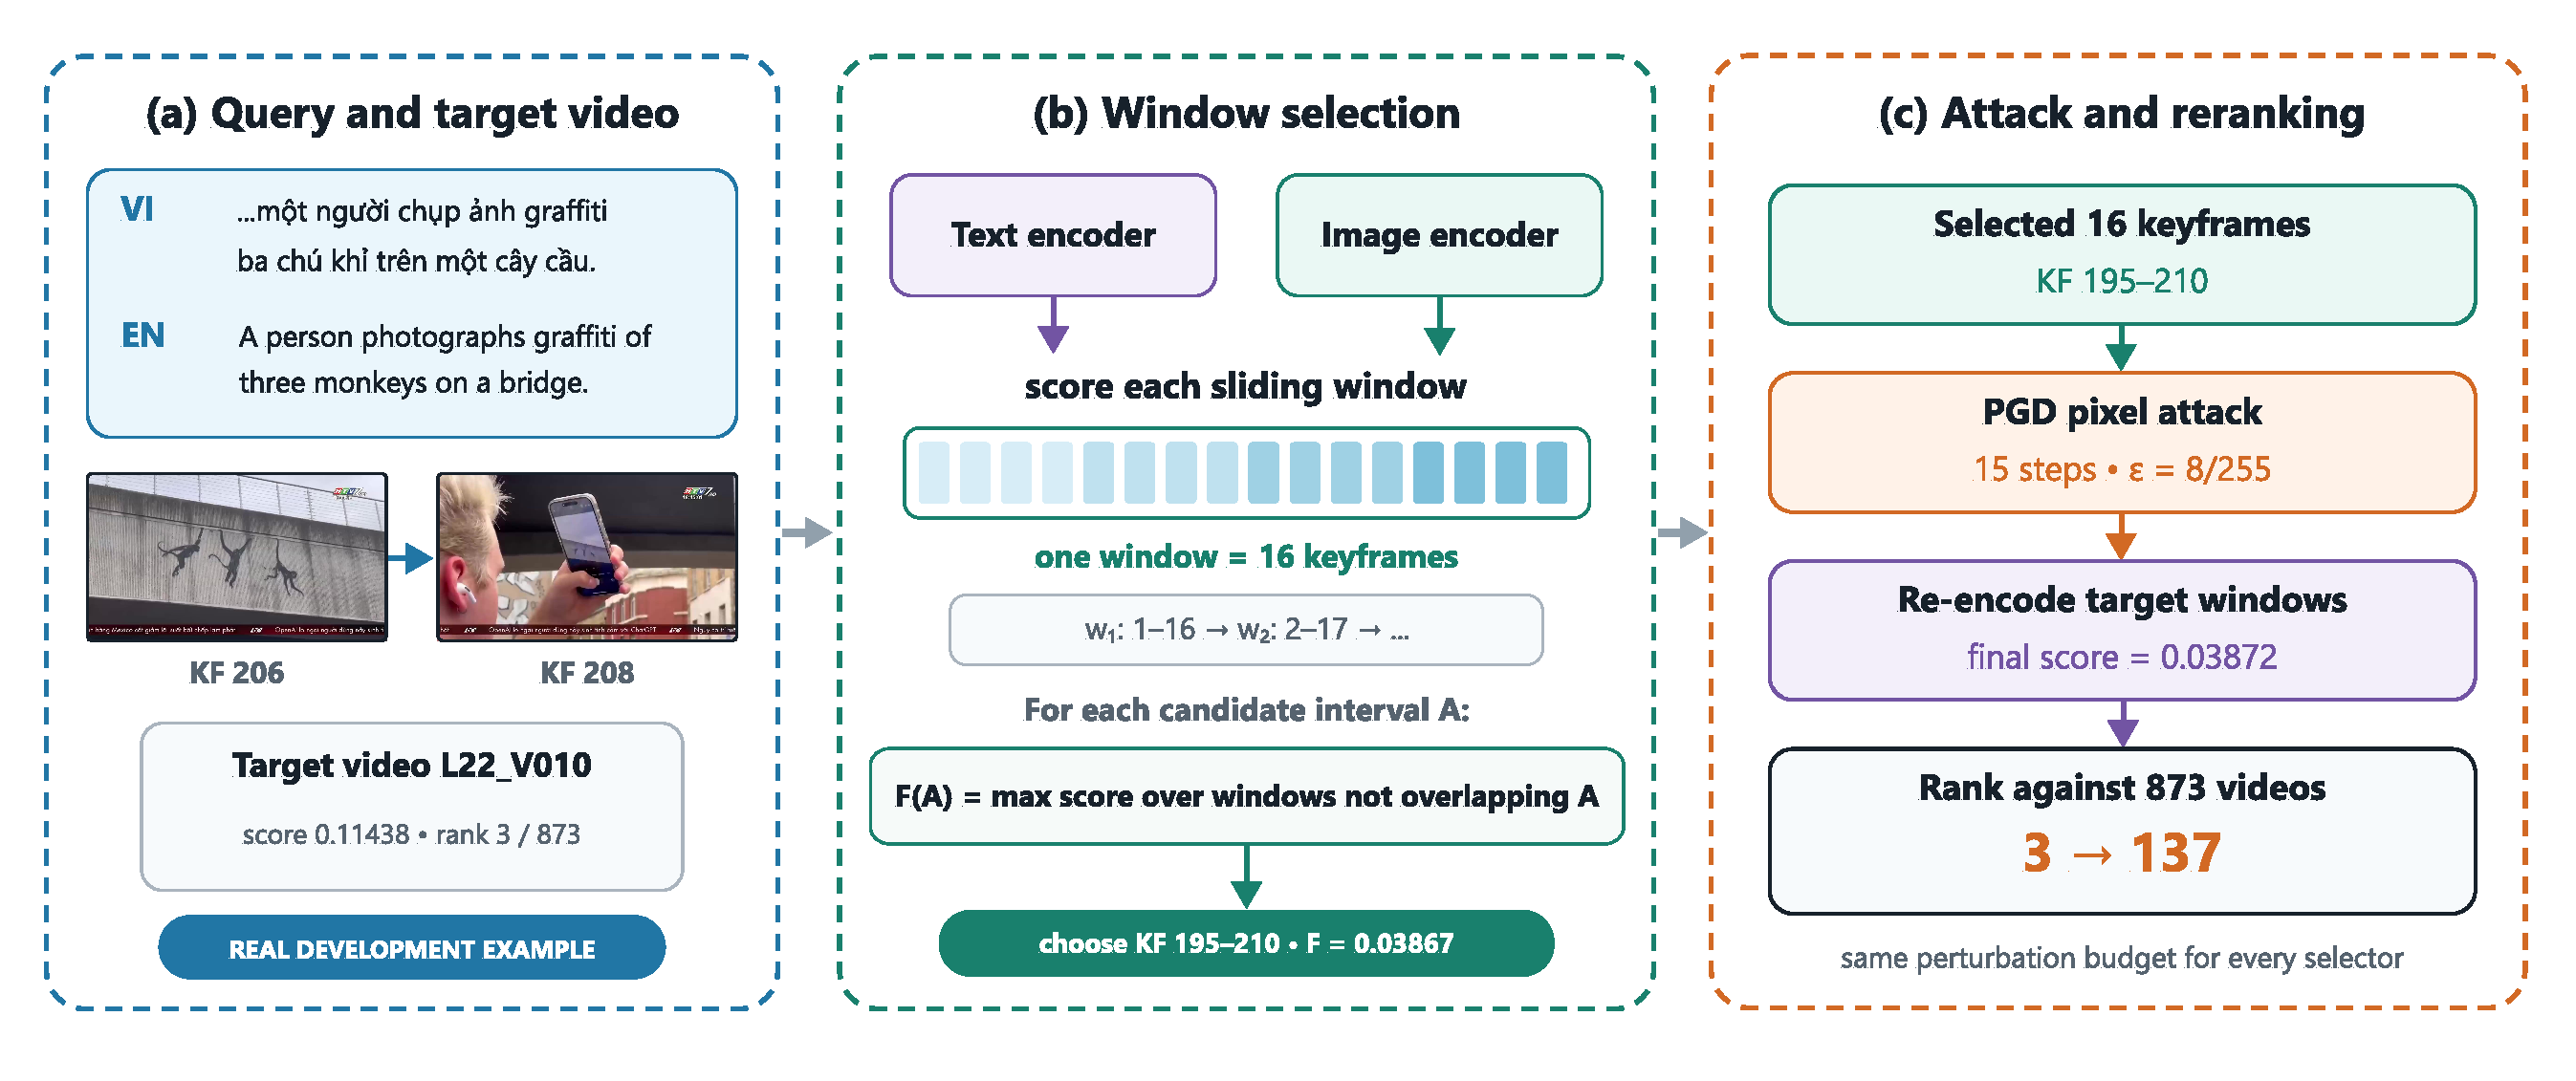
\includegraphics[width=\linewidth]{figures/ATTACK FRAMEWORK.pdf}
\caption{Attack framework: (a) query and target video, (b) editable interval selection, and (c) pixel optimization and reranking. The illustrated development example moves from rank 3 to rank 137.}
\label{fig:attack-framework}
\end{figure}

\subsection{Retrieval model}

Each video is represented by a temporally ordered keyframe sequence. Retrieval windows contain 16 sampled keyframes with stride one; their duration therefore depends on the sampling times. Videos with fewer than 16 keyframes are padded by repeating the last keyframe. All attacked targets contain at least 16 keyframes.

We use frozen SigLIP text and image encoders~\cite{zhai2023siglip} to obtain query and keyframe embeddings. Each query is represented by the normalized mean of its individually normalized English prompt embeddings. The prompts are fixed before evaluation and shared across clean retrieval and all attack methods. A query may have several prompts within its catalog record; Section~\ref{sec:queries-split} describes their construction. Each temporal window is represented by the normalized mean of its 16 keyframe embeddings, each normalized individually. The window score $c(q,w)$ is the cosine similarity between the query and window embeddings.

The video score is the largest score among all its windows:
\begin{equation}
s(q,V)=\max_{w\in\mathcal W(V)}c(q,w),
\end{equation}
where $q$ is the query, $V$ is a video, and $\mathcal W(V)$ is the set of its windows. Videos are ranked by descending score, with exact ties resolved by ascending video identifier. Higher numerical target ranks indicate stronger suppression.

\subsection{Threat model}

The attacker has white-box access to the frozen image encoder and its gradients. Edits are restricted to one interval of 16 consecutive sampled keyframes in the target video; the model, query, and all other videos remain fixed.

Pixel values lie in $[0,1]$, and perturbations satisfy an $\ell_\infty$ bound of $\epsilon=8/255$. Perturbed images are clipped to the valid pixel range, and keyframes outside the selected interval remain unchanged. Evaluation operates directly on the perturbed keyframes.

\subsection{Interval selection}

With a frame-independent encoder and identical preprocessing, changing frames in interval $A$ leaves every non-overlapping window unchanged. Partitioning the retrieval windows therefore gives
\begin{equation}
s_{\mathrm{adv}}(q,V;A,\delta)=\max\{F_{\mathrm{pix}}(A),G_{\mathrm{pix}}(A,\delta)\},
\label{eq:score-decomposition}
\end{equation}
where $F_{\mathrm{pix}}$ is the maximum clean pixel-encoded score over unaffected windows and $G_{\mathrm{pix}}$ is the maximum perturbed score over affected windows. The maximum of an empty unaffected set is $-\infty$. Thus, $F_{\mathrm{pix}}$ bounds the attainable score from below, regardless of the pixel optimizer. For example, an unaffected window scoring 0.75 prevents suppression below 0.75. This bound motivates interval selection, but does not guarantee the optimal final rank because affected windows may remain difficult to suppress.

For a possible editable interval $A_j$, we calculate the highest score among all windows that do not overlap it:
\begin{equation}
F(j)=\max_{w:\,w\cap A_j=\varnothing}\widehat c(q,w),
\end{equation}
Here $A_j$ contains the 16 positions starting at $j$, and $\widehat c$ is the clean similarity from saved embeddings. This cached unaffected floor is a proxy for $F_{\mathrm{pix}}$ in Eq.~\ref{eq:score-decomposition}; Section~\ref{sec:reranking} explains the encoding distinction. We examine every valid interval and choose the one with the smallest $F(j)$. Ties use the earliest interval. If an interval overlaps every window, we set $F(j)=-\infty$, so it is preferred over any interval with an unaffected window. If all intervals have this value, we select the earliest one.

We compare three selection rules:
\begin{enumerate}
\item \textbf{Target-centered.} Select the interval around the human-reviewed target keyframe, using seven positions before it and eight after it. At video boundaries, we shift the interval inward to keep 16 positions. Only this baseline receives the human-reviewed location of the relevant moment.
\item \textbf{Highest-score window.} Select the clean window with the largest query similarity; ties use the earliest window.
\item \textbf{Minimum unaffected floor.} Select the interval with the smallest value of $F(j)$.
\end{enumerate}

The minimum-floor rule reuses clean retrieval scores and adds selection work without extra PGD updates. Each update evaluates the affected windows, whose number can vary with interval position. Thus, matching the number of updates and pixel budget does not imply equal total runtime.

\subsection{Perturbation optimization}

After selecting the interval, we keep its location fixed. At each update, we find the highest-scoring window that overlaps the interval and use its gradient to lower its score; exact ties use the earliest window. We also penalize large differences between the pixel changes on neighboring keyframes. This smoothness term is
\begin{equation}
L_{\mathrm{smooth}}(\delta)=
\frac{\sum_{t=0}^{T-2}\|\delta_{t+1}-\delta_t\|_F^2}{(T-1)CHW},
\end{equation}
where $\delta_t$ is the change to keyframe $t$, $T$ is the full number of keyframes, and $C$, $H$, and $W$ are the image dimensions. Changes outside the selected interval are zero, so the term also covers the interval boundaries. Differences are measured between sampled-frame indices, rather than per second of elapsed video time; normalization uses the full sequence length.

The objective is the highest affected-window score plus $0.5L_{\mathrm{smooth}}$. We minimize it with projected gradient descent (PGD)~\cite{madry2018pgd}. The attack starts with zero changes and performs 15 updates. The first step size is $2/255$ and decreases linearly to 10\% of that value. Each update subtracts the step size times the sign of the objective gradient. We use the final iterate, without random restarts or selecting an earlier iterate. After each update, we set all changes outside the interval to zero and clip the remaining values to the pixel budget and valid image range. All three selection rules use exactly the same optimizer and budget.

\subsection{Full-corpus reranking}
\label{sec:reranking}

After the attack, we encode every window of the target video again. We replace the target's saved clean representation with these new representations, while the other 872 videos keep their validated clean representations. We then rank the target against the full collection.

Reranking uses the maximum over all freshly encoded target windows, including any affected or unaffected window that becomes dominant after optimization.

The clean rank and selection scores come from saved embeddings, whereas the final target score uses fresh pixel encoding. Numerical differences between them can contribute to changes from the clean rank. The unchanged-window argument assumes identical preprocessing and encoding, so the cached floor is a selection criterion rather than an exact numerical bound on the final pixel-evaluated score. All selectors share the same final encoding procedure. The reported evaluation does not isolate this difference with a zero-perturbation re-encoding control, so clean-to-attacked changes, including ASR, should be interpreted under this mixed cached/fresh protocol.

\section{Experimental Setup}

\subsection{Queries, targets, and split}
\label{sec:queries-split}

We use the Batch 1 video data available to participants in the Ho Chi Minh City AI Challenge (HCMC AI Challenge)~\cite{hcmcaic}. Each evaluation item contains a Vietnamese query, one locked target video, and temporal evidence for the relevant moment. We preserve the query wording and lock every query--target mapping before observing test attack results.

We report a prospective primary cohort and retain an earlier evaluation cohort for context. The earlier cohort contains 48 queries associated with 46 target videos; its results were already known before the prospective cohort was locked. The primary cohort began with 100 separately authored query--target records. A retrieval-based uniqueness audit sent flagged cases to human top-five review, after which four ambiguous records were excluded. We excluded three more records whose target videos overlapped the fixed 10-query development set. This left 93 locked queries on 93 target videos. No attack result from these 93 queries was observed before their targets, prompts, interval selections, and attack configuration were fixed. The revised extension protocol did not include a separate human hard-negative review or delayed self-audit. Every query is ranked against the same corpus of 873 videos.

The two cohorts use separately locked English prompt catalogs. For the primary cohort, the English wording was human-authored and hash-bound before retrieval; all 93 records fit the 64-token SigLIP context without chunking. The earlier 48-query catalog retains 32 existing prompt records and adds model translations for 16 records using pinned, deterministic decoding. The extension queries were authored from target-video content before retrieval feedback; they are not independent translations of organizer queries. The target location is used separately by the target-centered selector. The evaluated inputs are English prompt centroids, so the results do not measure direct Vietnamese-language retrieval.

\subsection{Fixed configuration}

The image and text encoders use OpenCLIP \texttt{ViT-B-16-SigLIP} with \texttt{webli} weights in OpenCLIP 3.3.0. Preprocessing resizes RGB images to $224\times224$ with bicubic interpolation and normalizes each channel with mean 0.5 and standard deviation 0.5. We constrain perturbations at the stored keyframe resolution to bound changes to the edited images. PGD backpropagates through the differentiable, antialiased bicubic resize and channel normalization; $\epsilon$ therefore specifies the pre-resize pixel budget. The retriever uses 16-keyframe windows with stride one. The frozen query representation, video collection, target mappings, sampling procedure, model, and attack configuration are shared by all three selection rules. The attack uses $\epsilon=8/255$, 15 PGD updates, and the first-order smoothness weight 0.5. These choices were fixed before the test run.

The primary evaluation contains $93\times3=279$ query--strategy executions. All 279 completed successfully. A subsequent CPU audit also verified all 144 execution records from the earlier cohort, for 423 verified executions and no failed or dropped runs across both cohorts.

Source code and reproduction materials are available at: \url{https://github.com/haruxne/ISARS}.

\subsection{Measurements and statistical tests}

We report mean and median target rank and mean reciprocal rank (MRR). Higher ranks and lower MRR indicate stronger suppression. Post-attack Recall@10 is the fraction of the 93 primary queries whose target appears in the first ten results after the attack.

Attack success rate at ten (ASR@10) considers only targets that were initially in the top ten. An attack succeeds when such a target moves below rank 10. There are 58 eligible queries in the primary cohort.

We assess image fidelity using peak signal-to-noise ratio (PSNR) and structural similarity (SSIM)~\cite{wang2004ssim}. To compare methods query by query, we report higher, tied, and lower rank counts. Confidence intervals use 10,000 bootstrap resamples at the target-video level~\cite{field2007bootstrap} and percentile 95\% intervals; the statistic remains query-weighted. The 93 primary queries have 93 distinct target videos, although shared content or query construction can still induce dependence. The intervals are marginal 95\% intervals for each comparison. We also report the planned two-sided exact sign tests for non-tied query pairs, with Bonferroni correction for two comparisons. These tests assume independent query-level signs; this correction does not apply to the bootstrap intervals. We report the primary cohort separately from the earlier cohort. A pooled 141-query analysis is descriptive and secondary because the earlier results were known before the primary cohort was locked.

\FloatBarrier
\section{Results}

\subsection{Overall retrieval results}

The cached clean Recall@10 was $58/93=0.624$ in the primary cohort, providing 58 eligible queries for ASR@10. Table~\ref{tab:test-results} reports the attacked results. The minimum-floor rule produced the largest mean rank, 65.91, compared with 64.26 for highest-score selection and 53.27 for target-centered selection. Its MRR was also the lowest at 0.178.

\begin{table}[!htbp]
\centering
\caption{Results on the 93-query prospective cohort. A larger rank and lower MRR mean that the target is harder to retrieve. R@10 denotes post-attack Recall@10. ASR@10 uses the 58 queries whose targets were initially in the top ten.}
\label{tab:test-results}
\small
\setlength{\tabcolsep}{3pt}
\begin{tabular}{lrrrrr}
\toprule
Selection & Mean rank & Median & MRR & R@10 & ASR@10 \\
\midrule
Target-centered          & 53.27 & 11 & 0.288 & 0.484 & 13/58 \\
Highest-score window     & 64.26 & 21 & 0.201 & 0.312 & 29/58 \\
Minimum floor (ours)     & 65.91 & 22 & 0.178 & 0.280 & 32/58 \\
\bottomrule
\end{tabular}
\end{table}

\subsection{Paired query-level comparison}

Figure~\ref{fig:primary-results} summarizes final target ranks and the paired outcomes for the primary cohort.

Compared with target-centered selection, our rule gave a higher target rank on 61 queries and the same rank on 32, with no lower ranks. Compared with highest-score selection, the counts were 19 higher, 74 tied, and zero lower. The median paired gains were three positions and zero positions, respectively. The second comparison therefore combines a modest average gain with frequent identical ranks.

The mean paired gain over target-centered selection was 12.65 positions, with a 95\% video-bootstrap interval of [7.87, 18.67]. The mean gain over highest-score selection was 1.66 positions, with an interval of [0.76, 2.78]. After Bonferroni correction, the exact sign-test $p$-values were $1.73\times10^{-18}$ and $7.63\times10^{-6}$. Each primary query has a distinct target video, so the video-cluster bootstrap has 93 clusters.

\begin{figure}[!htbp]
\centering
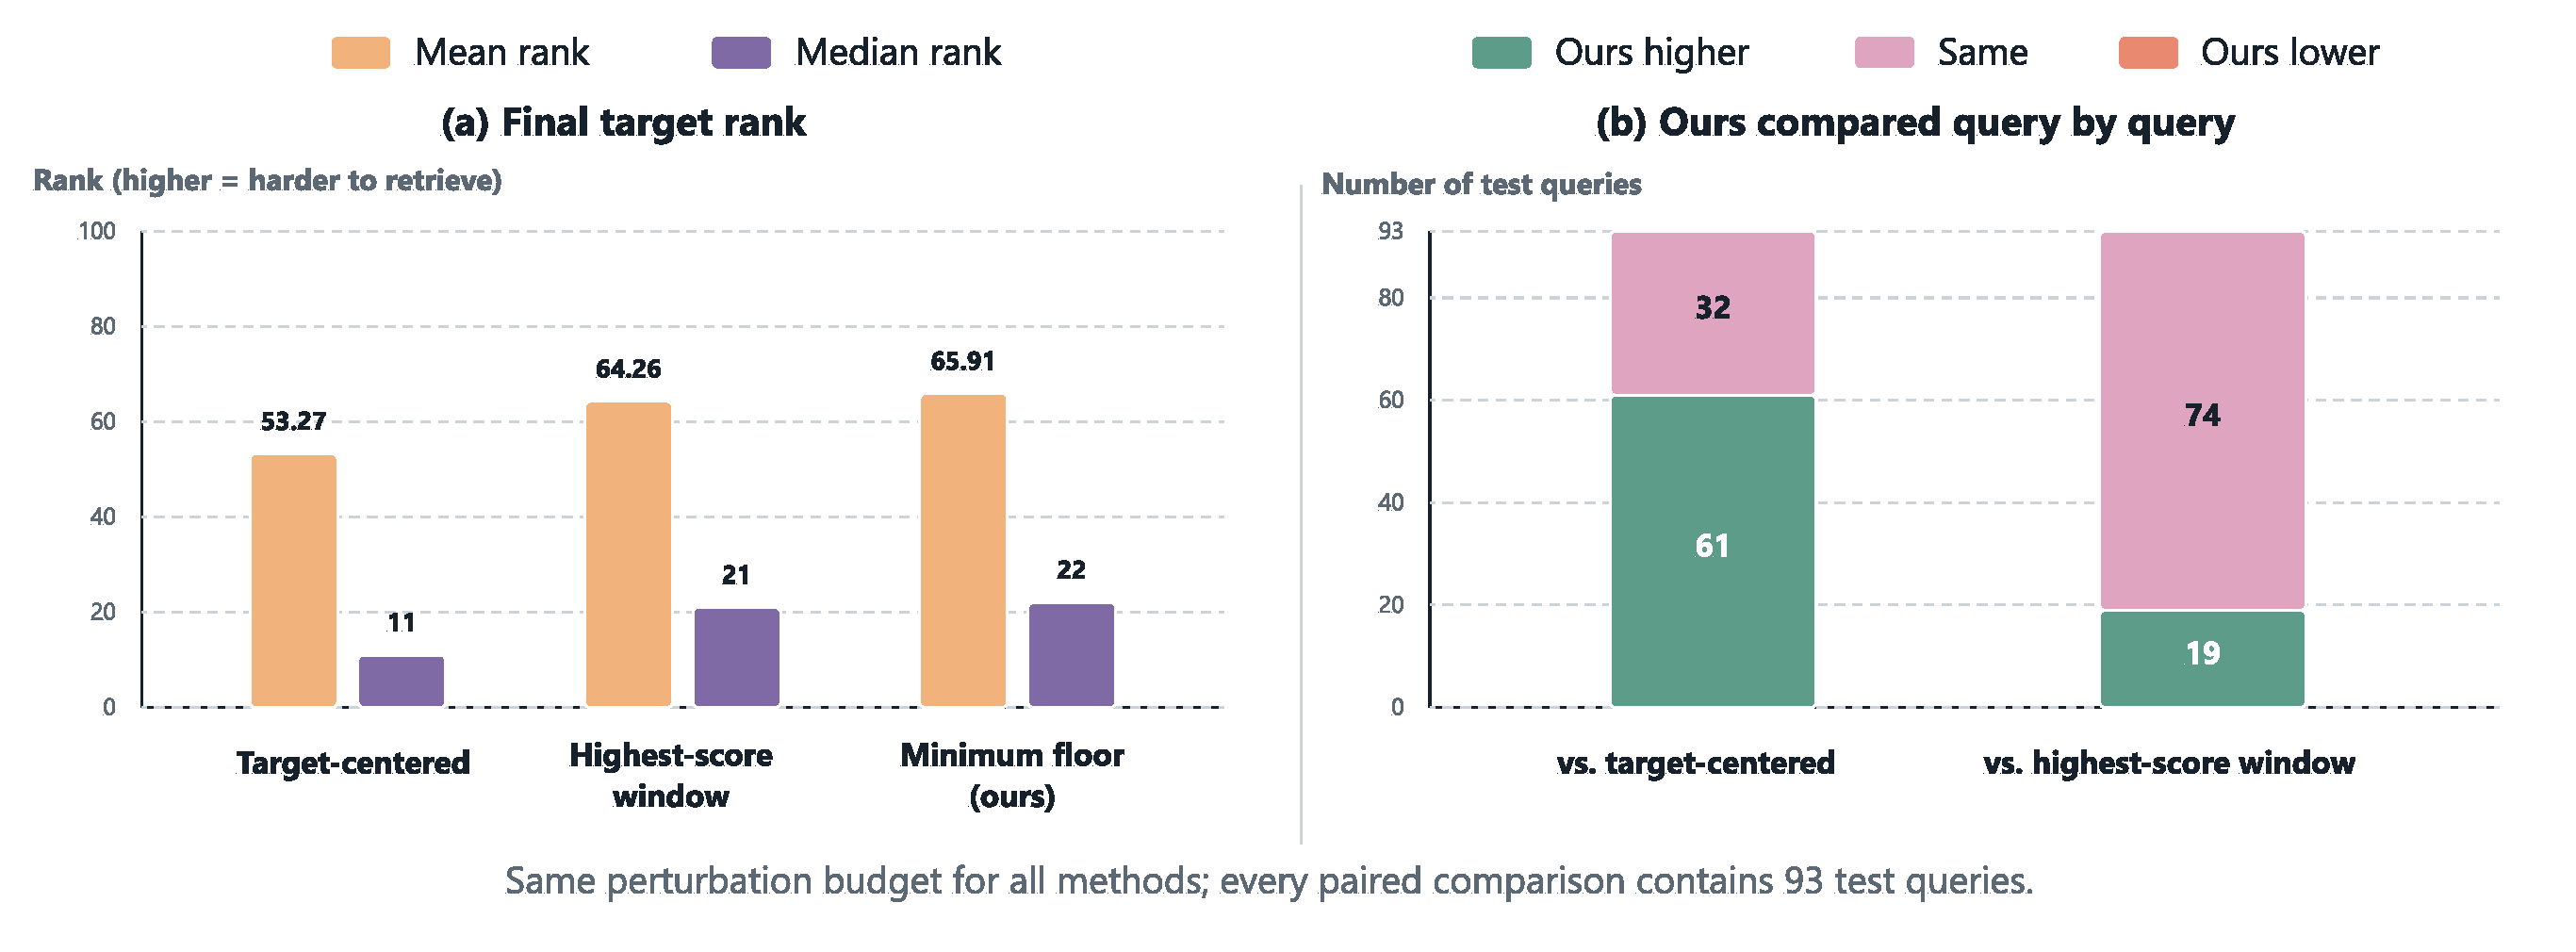
\includegraphics[width=\linewidth]{figures/RESULT.pdf}
\caption{Primary-cohort comparison under the same perturbation budget. (a) Mean and median final target ranks. (b) Query-level outcomes for minimum-floor selection relative to each baseline; neither comparison contains a lower-rank outcome.}
\label{fig:primary-results}
\end{figure}

\subsection{Top-ten attack success and image fidelity}

Our rule moved 32 of the 58 eligible targets out of the top ten, for ASR@10 of 55.17\%. Highest-score selection moved 29 of 58 (50.00\%), and target-centered selection moved 13 of 58 (22.41\%). Post-attack Recall@10 was correspondingly 0.280, 0.312, and 0.484. The advantage over highest-score selection is three additional successes in this cohort. We report this difference descriptively; the sign tests concern rank differences rather than binary attack success.

Table~\ref{tab:image-quality} reports image fidelity for each selector.
\begin{table}[!htbp]
\centering
\caption{Mean image-quality measurements over the evaluated sequences, including unchanged keyframes. Higher values indicate closer agreement with the original images.}
\label{tab:image-quality}
\begin{tabular}{lrr}
\toprule
Selection & PSNR (dB) & SSIM \\
\midrule
Target-centered & 55.91 & 0.99858 \\
Highest-score window & 55.85 & 0.99870 \\
Minimum floor (ours) & 56.70 & 0.99895 \\
\bottomrule
\end{tabular}
\end{table}

All methods yielded mean PSNR above 55 dB and mean SSIM above 0.998. These sequence-level averages include unchanged keyframes and reflect different selected content, so they do not establish a perceptual advantage on the edited keyframes.

\subsection{Earlier cohort and secondary pooled analysis}

The CPU audit reproduced the earlier 48-query results from their original authority records. On that cohort, mean ranks were 45.06, 70.17, and 86.65 for target-centered, highest-score, and minimum-floor selection. The minimum-floor comparison yielded higher/tied/lower counts of 24/23/1 and 15/32/1 against the two baselines. All three methods had ASR@10 of 12/29. These results provide historical context rather than a second prospective test.

Pooling both cohorts gives 141 queries on 130 target videos. In this secondary descriptive analysis, mean ranks were 50.48, 66.27, and 72.97, while the minimum-floor higher/tied/lower counts were 85/55/1 and 34/106/1. We keep the pooled result secondary because the earlier 48-query outcomes were observed before the 93-query protocol was locked.

\section{Discussion}

The results indicate that interval placement affects rank suppression in a retriever with maximum window aggregation. Both the annotated target moment and the highest-scoring window can leave strong temporal matches unaffected. The minimum-floor criterion explicitly accounts for these competing matches before pixel optimization.

The positive mean paired gains and video-cluster intervals support stronger average rank suppression on the prospectively locked cohort. The method also achieved the highest ASR@10, although the gain over highest-score selection was three of 58 eligible queries. Frequent rank ties, especially the 74 ties against highest-score selection, limit the magnitude of the claim. Identical selected intervals can produce identical attacks, while different intervals can still yield the same rank; the reported rank counts do not distinguish these mechanisms. When every interval overlaps every window, the floor criterion also reduces to its earliest-interval tie-break.

The study evaluates one prospectively locked 93-query cohort, one earlier 48-query cohort, one frozen frame-encoder retriever, and one video collection under white-box access. The cohorts are curated rather than random samples of all possible queries. The controlled construction exposes the role of maximum aggregation, but does not establish the same behavior in temporal video encoders or an entire competition retrieval system. Evaluation changes sampled keyframes rather than encoded videos; persistence after compression, black-box transfer, sparse retrieval, rank fusion, and later reranking remain outside the evidence. The cached/fresh encoding distinction in Section~\ref{sec:reranking} further limits the interpretation of absolute attack success.

\section{Ethical Considerations}

Adversarial retrieval attacks can be misused to hide relevant media from a search system. We study them to reveal a failure mode and support more robust retrieval. The attacker changes copies of keyframes from reviewed target videos in a controlled experiment. Queries, source records, and distractor videos remain unchanged. We report unsuccessful and tied cases so that the results do not overstate the attack's reliability.

\section{Conclusion}

We studied interval selection for adversarial rank suppression in a text-to-video retriever with maximum window aggregation. The evaluated rule selects a 16-keyframe interval by minimizing the maximum clean score among unaffected windows.

On the prospectively locked set of 93 evaluation queries, the rule increased mean target rank relative to target-centered and highest-score selection under a matched optimizer and pixel budget, without a lower rank on any paired query. It also produced the highest ASR@10, moving 32 of 58 eligible targets below rank ten. The modest mean gain and frequent ties relative to highest-score selection limit the result to this retriever and protocol. Future work will add a zero-perturbation re-encoding control and examine other retrieval architectures, black-box access, and encoded-video evaluation.

%
% ---- Bibliography ----
%
% BibTeX users should specify bibliography style 'splncs04'.
% Bibliography style 'splncs04' is recommended for LLNCS papers.
%
\bibliographystyle{splncs04}
\bibliography{references}
%
\end{document}
